\documentclass[10pt]{article}
\usepackage[utf8]{inputenc}
\usepackage[T1]{fontenc}
\usepackage{graphicx}
\usepackage[export]{adjustbox}
\graphicspath{ {./images/} }
\usepackage{amsmath}
\usepackage{amsfonts}
\usepackage{amssymb}
\usepackage[version=4]{mhchem}
\usepackage{stmaryrd}
\usepackage{multirow}

\title{S2I }

\author{}
\date{}


\begin{document}
\maketitle
\begin{center}
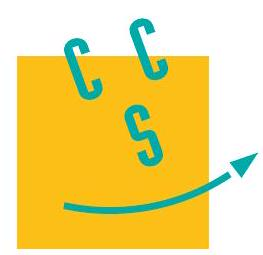
\includegraphics[max width=\textwidth]{2023_05_12_54c6a64d2ffce28d5c72g-01}
\end{center}

\section{Contexte}
Dans la volonté de rééducation à la marche des patients partiellement ou totalement paralysés au niveau des membres inférieurs, les exosquelettes de marche offrent une solution de plus en plus envisagée par les structures de soins. Si les technologies existantes permettent des séances de rééducation musculaire efficaces, elles n'offrent pour le moment que peu de possibilités d'amélioration dans la vie quotidienne des patients, du fait de la nécessité de la présence d'un personnel soignant formé à leur utilisation.

Il apparait ainsi qu'une solution permettant une plus grande autonomie des patients, que ce soit pour des séances de rééducation encadrées, ou pour leurs déplacements dans la vie quotidienne serait une grande avancée. Elle permettrait ainsi des fréquences, intensités et durées de séances plus en phase avec la pathologie de la personne équipée, tout en facilitant sa mobilité au quotidien.

Pensé pour minimiser le temps de formation pour le patient et le thérapeute, l'exosquelette Atalante (figure 1), développé par la société Wandercraft a pour volonté d'optimiser les séances de rééducation, et à terme d'aboutir à une solution permettant l'autonomie quasi totale du patient. En effet, ce système permet la verticalisation et des déplacements pouvant s'affranchir de toute dépendance à une tierce personne. De par sa liberté d'utilisation pour le patient, les bénéfices sont importants : possibilité de retours sensoriels, flexibilité de l'entrainement à la marche et à la course ou encore personnalisation des programmes proposés.
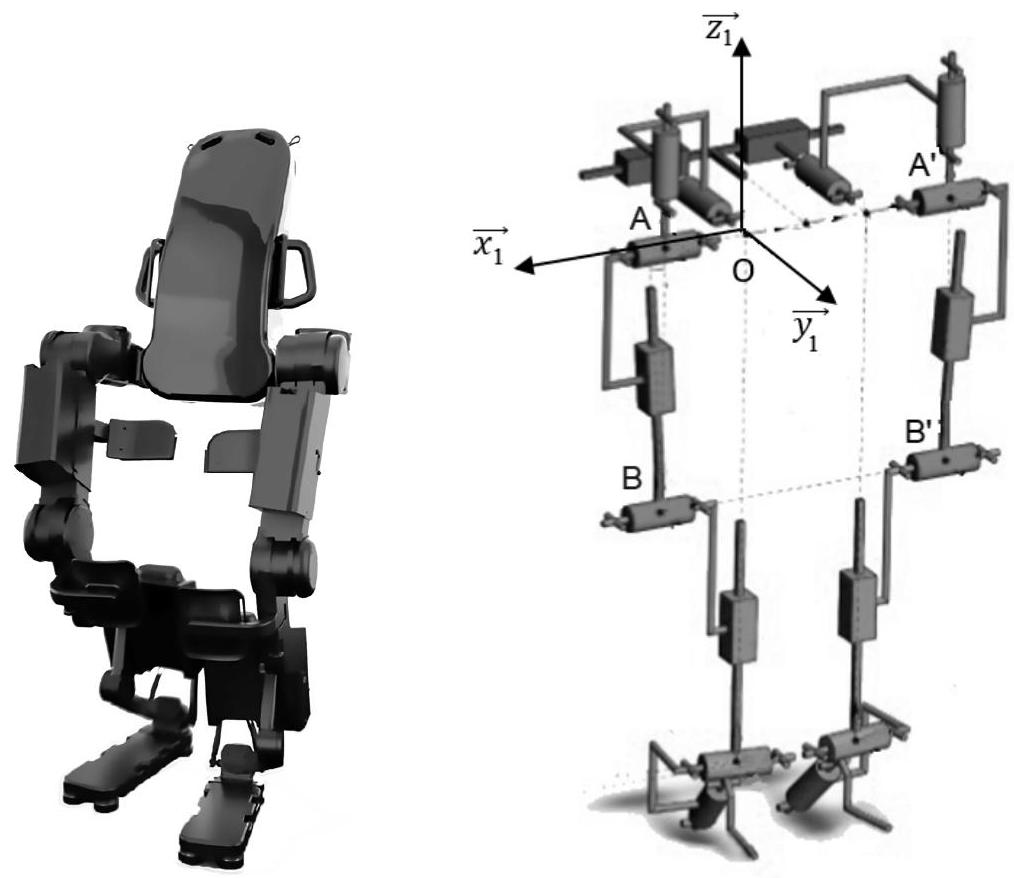
\includegraphics[max width=\textwidth, center]{2023_05_12_54c6a64d2ffce28d5c72g-01(1)}

Figure 1 Exosquelette Atalante et modélisation 3D associée

L'architecture de l'exosquelette autorise la complète autonomie des membres supérieurs du patient. De plus, le réglage rapide des dimensions des jambes et des tibias de l'exosquelette et une utilisation intuitive de son paramétrage permettent une utilisation plus aisée. Ainsi, associé avec la possibilité de variation de l'aide apportée par les différents actionneurs, cet équipement est en parfaite adéquation avec l'enchainement des séances de rééducation où les déplacements sont totalement pris en charge, quelles que soient la pathologie et la morphologie du patient.

Les exercices programmés par les thérapeutes s'articulent autour de deux stratégies thérapeutiques différentes, selon le handicap du patient :

\begin{itemize}
  \item la proprioception (sa propre perception) de la verticalité et de la marche pour les patients paraplégiques ou ayant des problèmes d'équilibre ;

  \item le renforcement musculaire pour les patients ayant subi un traumatisme important. Afin de permettre au patient de reproduire une marche comparable à celle d'un humain valide, et ce quel que soit l'exercice de rééducation préprogrammé, l'exosquelette Atalante possède douze degrés de liberté, six par jambe, et chaque mobilité est contrôlée par un actionneur électrique.

\end{itemize}

L'ensemble de l'étude menée dans ce sujet se limitera à une marche en ligne droite (figure 3), dans le plan sagittal tel que défini figure 2.

La loi de commande des actionneurs associés aux différentes articulations est donc conditionnée par :

\begin{itemize}
  \item les trajectoires des différents membres lors de la marche, prédéterminées par un serveur extérieur lors de la prise de mesures du patient ;

  \item la stabilisation du patient lors de la marche;

  \item la rééducation musculaire du patient, selon un protocole dicté par le thérapeute.

\end{itemize}

Le cahier des charges partiel de l'exosquelette à vérifier dans ce sujet est fourni en annexe A.

\begin{center}
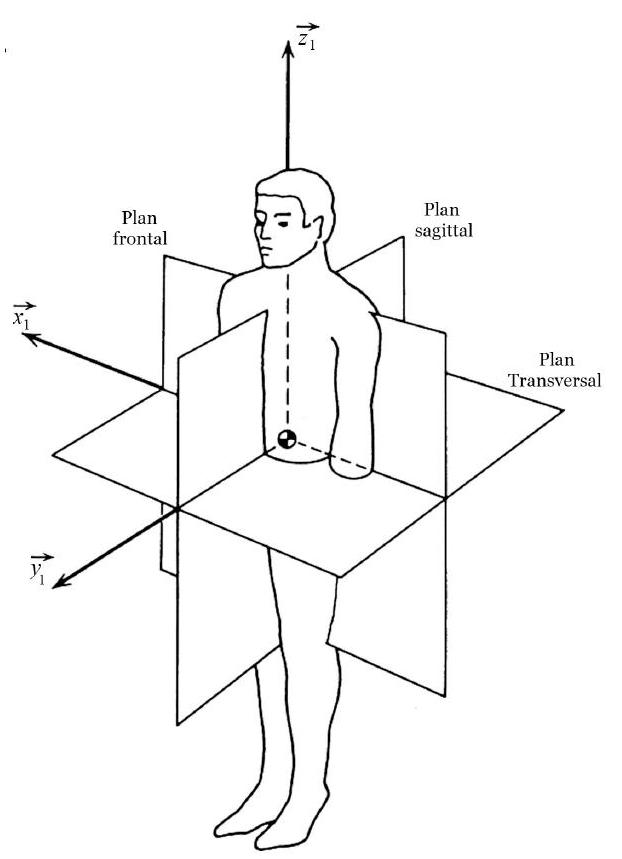
\includegraphics[max width=\textwidth]{2023_05_12_54c6a64d2ffce28d5c72g-02}
\end{center}

Figure 2 Description des plans d'évolution

\begin{center}
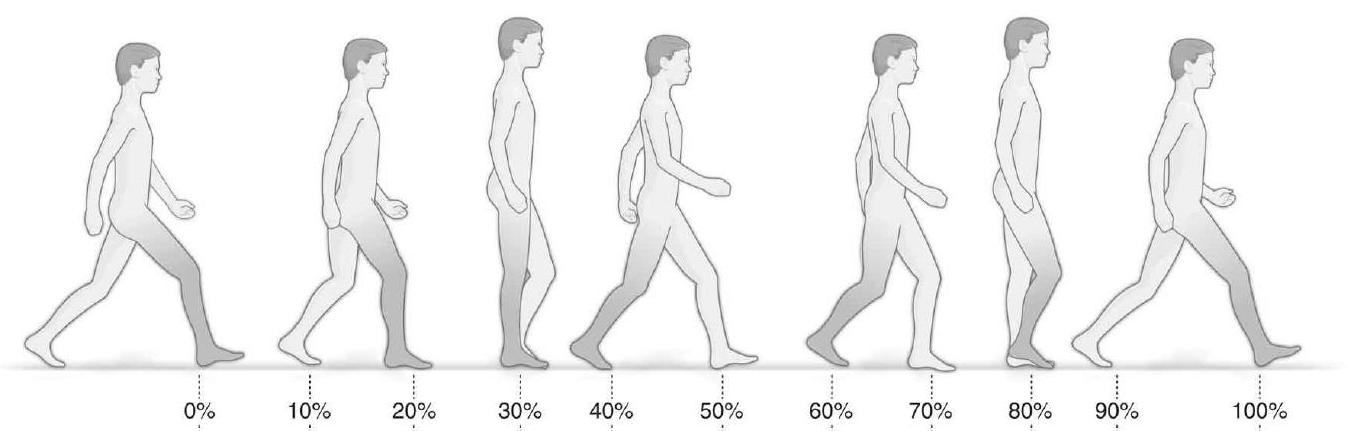
\includegraphics[max width=\textwidth]{2023_05_12_54c6a64d2ffce28d5c72g-02(1)}
\end{center}

Figure 3 Description d'une foulée en ligne droite

\section*{I Mise en évidence de la problématique lors d'une marche en ligne droite }
\begin{abstract}
Objectif Reformuler le cahier des charges global en termes de précision de façon à l'exprimer pour chacun des axes et mettre en évidence la nécessité de la prise en compte du couplage entre les axes dans la synthèse de la loi de commande.
\end{abstract}

En phase de rééducation à la proprioception de la verticalité et de la marche, il est nécessaire d'éviter la chute du patient. Des essais, menés sur des humains valides, ont permis de mettre en avant que lors d'une marche en ligne droite, une erreur de positionnement du talon de $\pm 5 \mathrm{~mm}$ risque d'amener à un déséquilibre, et donc à une chute (exigence 1.2.1.1, annexe A). Il est donc nécessaire de déterminer l'erreur de positionnement angulaire admissible sur chacun des axes de l'exosquelette pour éviter cette chute.

Dans toute l'étude, les hypothèses et notations seront les suivantes (figure 4) :

\begin{itemize}
  \item l'étude est menée dans le plan sagittal $\left(A, \vec{y}_{1}, \vec{z}_{1}\right)$, où $\vec{z}_{1}$ est vertical ascendant ;

  \item les différentes caractéristiques de dimension, masse et inertie des différents solides sont précisées annexe B ;

  \item le buste 1 étant animé d'un mouvement de translation rectiligne uniforme par rapport au référentiel terrestre, il est considéré comme galiléen ;

  \item l'étude se limite à la partie de la marche pour laquelle une des deux jambes est totalement décollée du sol (de $70 \%$ à $100 \%$ de la foulée sur la figure 3) ;

  \item le buste 1 est en liaison pivot d'axe $\left(A, \vec{x}_{1}\right)$ avec la cuisse 2 ; on note $\theta_{1}=\left(\vec{y}_{1}, \vec{y}_{2}\right)=\left(\vec{z}_{1}, \vec{z}_{2}\right)$;

  \item l'ensemble \{pied+tibia 3 , considéré comme solidaire, est en liaison pivot d'axe $\left(B, \vec{x}_{1}\right)$ avec la cuisse 2 ; on note $\theta_{2}=\left(\vec{y}_{2}, \vec{y}_{3}\right)=\left(\vec{z}_{2}, \vec{z}_{3}\right)$;

  \item les liaisons décrites précédemment sont supposées parfaites.
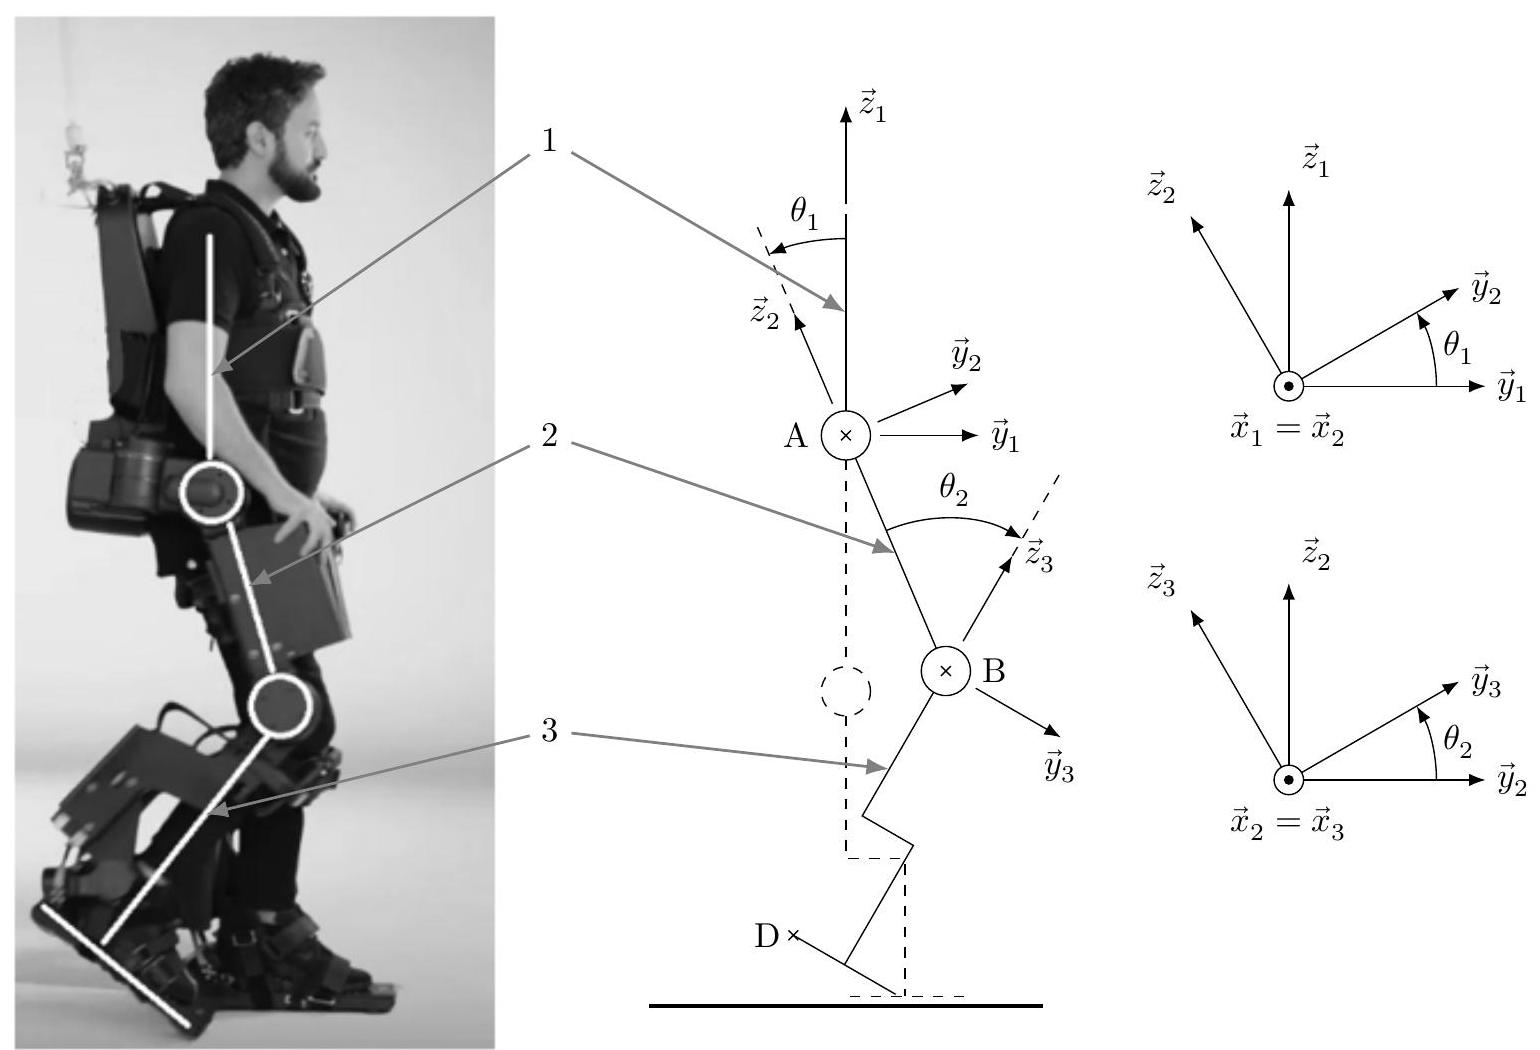
\includegraphics[max width=\textwidth, center]{2023_05_12_54c6a64d2ffce28d5c72g-03}

\end{itemize}

Figure 4 Modélisation utilisée pour la marche en ligne droite

Les positions des différents axes sont asservies à une consigne de référence afin d'obtenir la position désirée pour le point $D$ caractérisant la pointe du talon. Le cahier des charges impose que la position dans l'espace du point $D$ par rapport au point $A$ doive être celle désirée, avec une incertitude maximale de $S_{D}=5 \mathrm{~mm}$. On pose :

$$
\overrightarrow{A D}=Y \vec{y}_{1}+Z \vec{z}_{1}
$$

Q 1. Déterminer les expressions de $Y$ et $Z$, en fonction de $\theta_{1}, \theta_{2}, L_{2}$ et $L_{3}$.

L'erreur de positionnement du talon est modélisée par une variation autour d'une position connue. Cette position est paramétrée par les coordonnées $Y_{0}$ et $Z_{0}$ pour le point $D$, et par des angles $\theta_{1,0}$ et $\theta_{2,0}$ pour les liaisons pivots. Ce paramétrage se traduit, pour une variation angulaire $\Delta_{\theta}$, considérée égale sur chacun des axes, à des variations de position, $\Delta_{Y}$ et $\Delta_{Z}$, du point $D$. On suppose $\Delta_{\theta}$ faible, proche de 0 .

Q 2. À l'aide du résultat de la question 1, écrit à la position $\left(Y_{0}, Z_{0}\right)$, puis à la position $\left(Y_{0}+\Delta_{Y}, Z_{0}+\Delta_{Z}\right)$, déterminer les expressions de $\Delta_{Y}$ et $\Delta_{Z}$, en fonction de $\theta_{1,0}, \theta_{2,0}, \Delta_{\theta}, L_{2}$ et $L_{3}$.

Q 3. Déterminer alors $\Delta_{Y Z}$, la norme de la variation de positionnement total du point $D$ dans le plan $\left(\vec{y}_{1}, \vec{z}_{1}\right)$, en fonction de $\theta_{2,0}, \Delta_{\theta}, L_{2}$ et $L_{3}$.

Le résultat de la question précédente permet alors de relier l'erreur de position du talon $S_{D}$ à l'erreur de position sur les axes $S_{\theta}$, en considérant $\Delta_{Y Z}=S_{D}$ et $\Delta_{\theta}=S_{\theta}$. La figure 5 donne les évolutions sur un pas de marche de $S_{D}$ pour plusieurs valeurs de $S_{\theta}$.

Q 4. À partir de la figure 5, déterminer, parmi les valeurs proposées, l'erreur maximale admissible sur les axes $S_{\theta, \max }$ de l'exosquelette Atalante afin d'éviter la chute du patient.

Quel que soit le résultat trouvé à la question précédente, une erreur maximale admissible de 0,01 rad pour chacun des axes sera considérée pour la suite.

Afin de respecter l'exigence sur l'erreur maximale admissible, des asservissements de position et de vitesse ont été élaborés pour chacun des axes sans prendre en compte l'éventuelle influence du couplage entre les axes.

Des essais ont alors été effectués afin de mesurer l'évolution réelle des angles de chaque axe par rapport à la trajectoire visée. La figure 6 montre l'évolution de l'erreur pour l'axe de hanche sagittal de la jambe gauche lors d'une marche en ligne droite.

Q 5. À partir de la figure 6 et en justifiant la réponse, conclure sur la capacité des asservissements réalisés sans prise en compte du couplage entre les axes à respecter l'exigence 1.2.1.1.
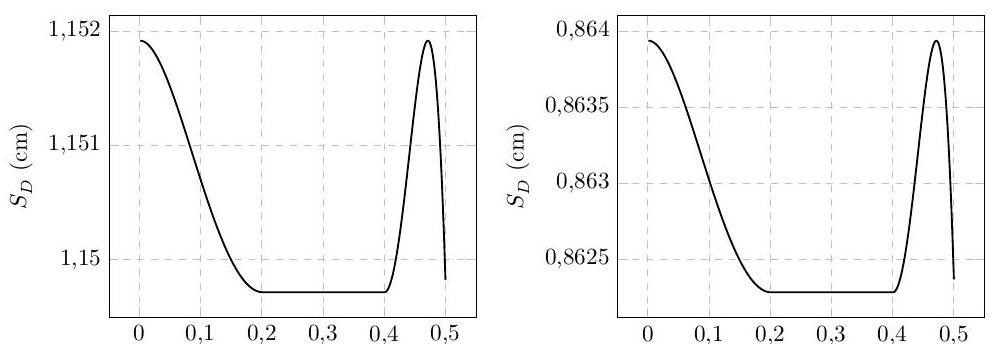
\includegraphics[max width=\textwidth, center]{2023_05_12_54c6a64d2ffce28d5c72g-04(2)}

temps (s)

\begin{center}
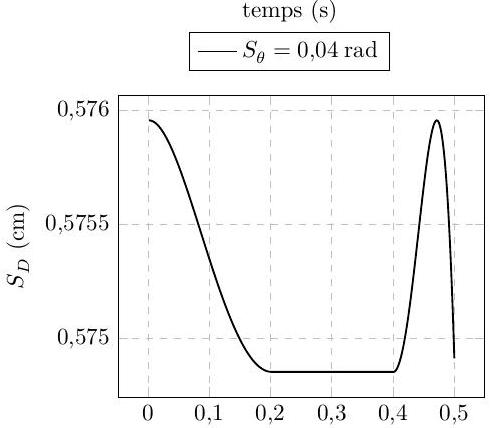
\includegraphics[max width=\textwidth]{2023_05_12_54c6a64d2ffce28d5c72g-04}
\end{center}

temps (s)

\begin{center}
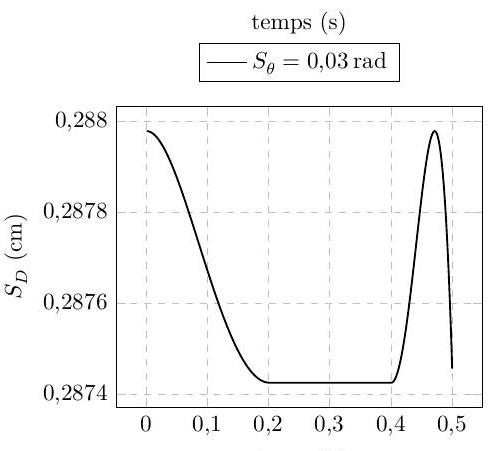
\includegraphics[max width=\textwidth]{2023_05_12_54c6a64d2ffce28d5c72g-04(4)}
\end{center}

temps (s)
$-S_{\theta}=0,02 \mathrm{rad}$

\begin{center}
\begin{tabular}{c}
temps (s) \\
$-S_{\theta}=0,01 \mathrm{rad}$ \\
\hline
\end{tabular}
\end{center}

Figure 5 Évolution de $S_{D}$ sur un pas de marche

\begin{center}
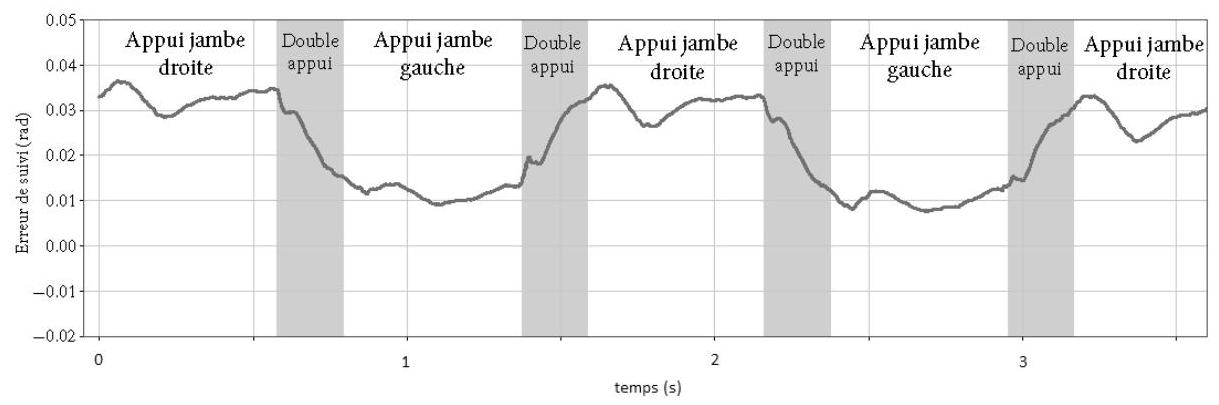
\includegraphics[max width=\textwidth]{2023_05_12_54c6a64d2ffce28d5c72g-04(3)}
\end{center}

Figure 6 Évolution de l'erreur pour l'axe de hanche sagittal de la jambe gauche

La question précédente met en avant la nécessité d'adopter une démarche de commande globale qui tient compte du couplage entre les axes. Le cahier des charges partiel de l'exosquelette concerné par cette étude (annexe A) fait apparaitre les deux exercices envisagés dans l'utilisation de l'exosquelette (renforcement musculaire et rééducation à la proprioception de la verticalité et de la marche).

Pour cela la structure envisagée de la commande s'appuie sur la figure 7 et peut être décomposée en :

\begin{itemize}
  \item un directeur de commande haut niveau (non étudié dans ce sujet). Il permet de générer en temps réel les consignes de trajectoire, ou de situation de rééducation à l'arrêt, pour chacun des axes. On suppose que ce directeur de commande, implémenté sur le buste de l'exosquelette, détermine les différentes consignes de trajectoire de manière parfaite ;

  \item une boucle interne (non linéaire). Elle a pour but de générer les actions mécaniques sur chacun des axes en fonction de la configuration d'évolution de l'exosquelette.

\end{itemize}

\begin{center}
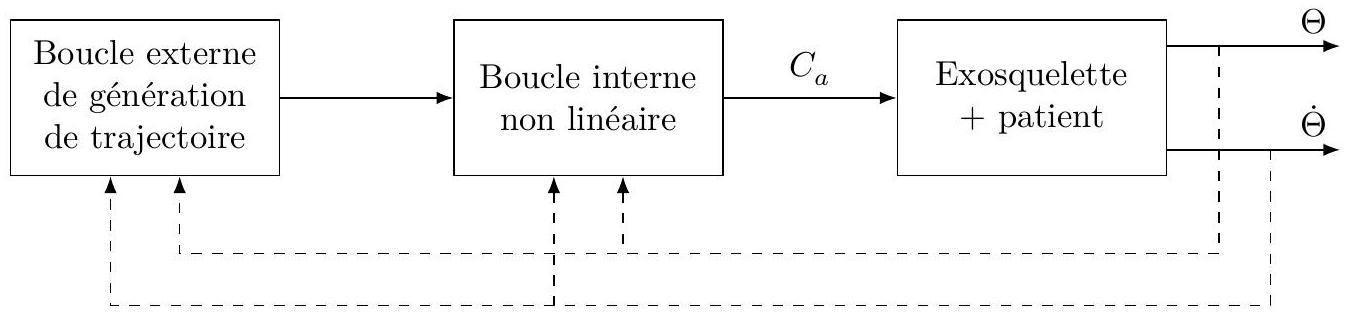
\includegraphics[max width=\textwidth]{2023_05_12_54c6a64d2ffce28d5c72g-04(1)}
\end{center}

Figure 7 Structure de commande choisie

Sur cette figure, $\Theta$ représente l'ensemble des positions angulaires des différents axes de l'exosquelette, et $C_{a}$ l'ensemble des actions mécaniques appliquées sur les différents axes.

La conception de cette commande nécessite de disposer d'un modèle dynamique de l'exosquelette. La définition et l'analyse de ce modèle dynamique seront réalisées dans la partie II. Il sera ensuite exploité dans la partie III pour la conception des lois de commande. La loi de commande dans le cas d'exercices de renforcement musculaire sera entièrement déterminée et celle dans le cas d'exercices de rééducation à la proprioception de la verticalité et de la marche sera analysée.

La partie IV permettra une synthèse des études menées.

\section{II Élaboration et analyse d'un modèle dynamique de l'exosquelette}
Définir un modèle dynamique de l’exosquelette et montrer la nécessité de mettre en place un asservissement

Afin d'élaborer une commande pour l'exosquelette, il est nécessaire au préalable de définir un modèle dynamique représentatif de son comportement. Seule la commande des articulations sagittales de hanche et de genou d'une jambe lorsqu'elle est décollée du sol (figure 7 et hypothèses associées) sera considérée ici (cas de la marche en ligne droite) avec les hypothèses et notations supplémentaires suivantes, en plus de celles énoncées à la partie précédente :

\begin{itemize}
  \item la liaison pivot entre 1 et 2 est équipée d'un actionneur dont le couple de sortie (appliqué par 1 sur 2 ) est noté $C_{1}$;

  \item la liaison pivot entre 2 et 3 est équipée d'un actionneur dont le couple de sortie (appliqué par 2 sur 3 ) est noté $C_{2}$;

  \item les différentes caractéristiques géométriques, de masses et d'inerties sont données en annexe B ;

  \item on note respectivement $C_{\text {genou }}$ et $C_{\text {hanche }}$, les couples appliqués par le patient au niveau des articulations de genou et de hanche.

\end{itemize}

Le modèle dynamique proposé sera explicité pour mettre en évidence la nécessité d'un asservissement et par la suite (partie III), permettre l'élaboration de la loi de commande globale de l'exosquelette.

\section{II.A - Comportement dynamique de l'exosquelette}
On pose pour la suite : $\overrightarrow{B G_{3}}=-L_{0} \vec{z}^{\prime}$. On note $\alpha$ l'angle entre $\vec{z}^{\prime}{ }_{3}$ et $\vec{z}_{3}: \alpha=\left(\vec{y}_{3}, \vec{y}^{\prime}{ }_{3}\right)=\left(\vec{z}_{3}, \vec{z}^{\prime}{ }_{3}\right)$.

Q 6. Déterminer les expressions de $L_{0}$ et $\alpha$ en fonction de $l_{0}, L_{3}$ et $l_{3}$, puis calculer leurs valeurs numériques.

Q 7. Déterminer l'expression de l'accélération du point $G_{3}$ (cf. annexe B et question 6) appartenant à l'ensemble \{pied+tibia\} 3 dans son mouvement par rapport au buste 1 , en fonction de $L_{0}, L_{2}, \theta_{1}, \theta_{2}$ et leurs dérivées temporelles.

Q 8. Déterminer l'expression de la projection suivant $\vec{x}_{1}$ du moment dynamique en $A$ de l'ensemble $\{$ pied+tibia $\}$ 3 dans son mouvement par rapport au buste $1, \vec{\delta}_{A, 3 / 1} \cdot \vec{x}_{1}$, sous la forme :

$$
\vec{\delta}_{A, 3 / 1} \cdot \vec{x}_{1}=A_{1} \ddot{\theta}_{1}+A_{2} \ddot{\theta}_{2}+A_{3} \dot{\theta}_{1}^{2}+A_{4}\left(\dot{\theta}_{1}+\dot{\theta}_{2}\right)^{2}
$$

Préciser les expressions littérales de $A_{1}, A_{2}, A_{3}$ et $A_{4}$ en fonction des différentes caractéristiques géométriques, de masses et d'inerties de l'exosquelette.

Q 9. Proposer une démarche permettant de déterminer l'expression de $C_{1}$, l'action mécanique exercée sur la cuisse 2 par l'actionneur correspondant. Préciser le(les) ensemble(s) isolé(s), le(s) bilan(s) des actions mécaniques extérieurs, le(s) théorème(s) utilisé(s) et la(les) équation(s) utile(s).

Q 10. Déterminer l'expression de $C_{1}$ en fonction de $\theta_{1}, \theta_{2}$, leurs différentes dérivées, de $C_{\text {hanche }}$ et des différentes caractéristiques géométriques, de masses et d'inerties de l'exosquelette.

D'une manière similaire aux questions précédentes, l'application du principe fondamental de la dynamique à l'ensemble \{pied+tibia\} 3 permet d'obtenir l'expression de $C_{2}$, le couple fourni par l'actionneur de genou sagittal :

$$
C_{2}=\left[I_{x 3}+m_{3} L_{0}^{2}\right]\left(\ddot{\theta}_{1}+\ddot{\theta}_{2}\right)+m_{3} L_{2} L_{0}\left[\ddot{\theta}_{1} \cos \left(\theta_{2}+\alpha\right)+\dot{\theta}_{1}^{2} \sin \left(\theta_{2}+\alpha\right)\right]+m_{3} g L_{0} \sin \left(\theta_{2}+\theta_{1}+\alpha\right)-C_{\text {genou }}
$$

Q 11. Déduire des deux équations précédentes que le modèle dynamique considéré peut s'écrire sous la forme matricielle suivante :

$$
\left(\begin{array}{l}
C_{1} \\
C_{2}
\end{array}\right)=M_{1}\left(\begin{array}{c}
\ddot{\theta}_{1} \\
\ddot{\theta}_{2}
\end{array}\right)+M_{2}\left(\begin{array}{c}
\dot{\theta}_{1} \\
\dot{\theta}_{2}
\end{array}\right)+C+M_{3}\left(\begin{array}{c}
C_{\text {hanche }} \\
C_{\text {genou }}
\end{array}\right)
$$

où $C$ est une matrice colonne et $M_{1}, M_{2}$ et $M_{3}$ sont des matrices $2 \times 2$. Donner l'expression littérale des coefficients de $C, M_{1}, M_{2}$ et $M_{3}$ par des relations non linéaires des paramètres de mouvement $\left(\theta_{1}, \theta_{2}\right)$, leurs dérivés premières et des différentes caractéristiques géométriques, de masses et d'inerties du problème.

\section{II.B - Analyse du modèle dynamique}
Le modèle dynamique déterminé à la question 11 étant couplé et non linéaire, un modèle linéarisé sera exploité afin de faciliter la synthèse de la loi de commande.

Autour de la position pour laquelle le pied se décolle du sol $\left(\theta_{1}=0, \theta_{2}=-35^{\circ}\right)$, le modèle dynamique linéarisé est :

$$
C_{a}=\left(\begin{array}{cc}
3,4 & 2,6 \\
2,6 & 1,9
\end{array}\right) \ddot{\Theta}+\left(\begin{array}{cc}
-11,5 & -19,2 \\
7,7 & 0
\end{array}\right) \dot{\Theta}+\left(\begin{array}{cc}
108,2 & 5,2 \\
15,9 & 17,1
\end{array}\right) \Theta-C_{p}
$$

Dans cette relation, on note :

$-\Theta=\left(\begin{array}{l}\theta_{1} \\ \theta_{2}\end{array}\right)$, les coordonnées angulaires des articulations

$-C_{p}=\left(\begin{array}{c}C_{\text {hanche }} \\ C_{\text {genou }}\end{array}\right)$, les actions mécaniques exercées par le patient ;

$-C_{a}=\left(\begin{array}{c}C_{1} \\ C_{2}\end{array}\right)$, les actions mécaniques générées par les actionneurs.

$\Theta_{1}(p), \Theta_{2}(p), C_{1}(p), C_{2}(p), C_{\text {hanche }}(p)$ et $C_{\text {genou }}(p)$ représentent les transformées de Laplace de, respectivement, $\theta_{1}(t), \theta_{2}(t), C_{1}(t), C_{2}(t), C_{\text {hanche }}(t)$ et $C_{\text {genou }}(t)$. Pour la question suivante, on considère que seul l'actionneur de l'axe de genou est actif $\left(C_{\text {hanche }}=C_{\text {genou }}=C_{1}=0\right)$ et que les conditions initiales sont nulles.

Q 12. Déterminer les valeurs numériques des coefficients $a_{i}$ et $b_{i}$ tels que la fonction de transfert $H_{L 4}(p)=$ $\frac{\Theta_{2}(p)}{C_{2}(p)}$ s'écrive :

$$
H_{L 4}(p)=\frac{a_{0}+a_{1} p+a_{2} p^{2}}{1+b_{1} p+b_{2} p^{2}+b_{3} p^{3}+b_{4} p^{4}}
$$

En poursuivant cette démarche, il est alors possible de mettre le modèle dynamique sous la forme de la figure 8 , faisant apparaitre le couplage entre les axes.

\begin{center}
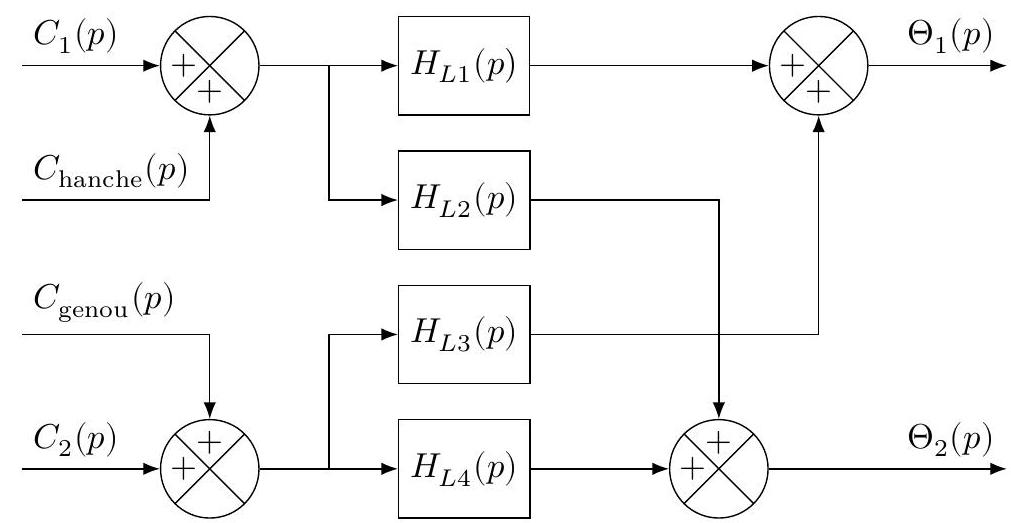
\includegraphics[max width=\textwidth]{2023_05_12_54c6a64d2ffce28d5c72g-06}
\end{center}

Figure 8 Représentation du modèle dynamique linéarisé

La fonction de transfert $H_{L 4}(p)$, une fois les polynômes du numérateur et dénominateur factorisés, s'écrit :

$$
H_{L 4}(p)=K_{L 4} \frac{\left(p-z_{1}\right)\left(p-z_{2}\right)}{\left(p-p_{1}\right)\left(p-p_{2}\right)\left(p^{2}+0,1 p+4,9\right)}
$$

avec $z_{1}=1,7+2,2 i, z_{2}=1,7-2,2 i, p_{1}=-23,6$ et $p_{2}=50,5$.

Q 13. Au regard de cette fonction de transfert, justifier le besoin de la mise en place d'un asservissement pour l'exosquelette.

\section{Conception et analyse de lois de commande de l'exosquelette}
Le modèle dynamique multivariable de l'exosquelette linéarisé autour d'une position donnée, déterminé à la partie précédente, est exploité pour l'élaboration et l'analyse des lois de commande de l'exosquelette. La boucle interne non linéaire (figure 7) doit permettre au système de respecter le cahier des charges (annexe A) en aboutissant, sur les différents axes considérés, à des actions mécaniques permettant la réalisation de l'exercice thérapeutique envisagé.

Dans les faits, des actionneurs électriques sont présents sur chacun des axes de façon à générer les actions mécaniques. La structure de commande peut alors être détaillée par la figure 9 , où $C_{\text {ref }}$ représente l'ensemble des valeurs cibles d'actions mécaniques appliquées aux différents axes.

\begin{center}
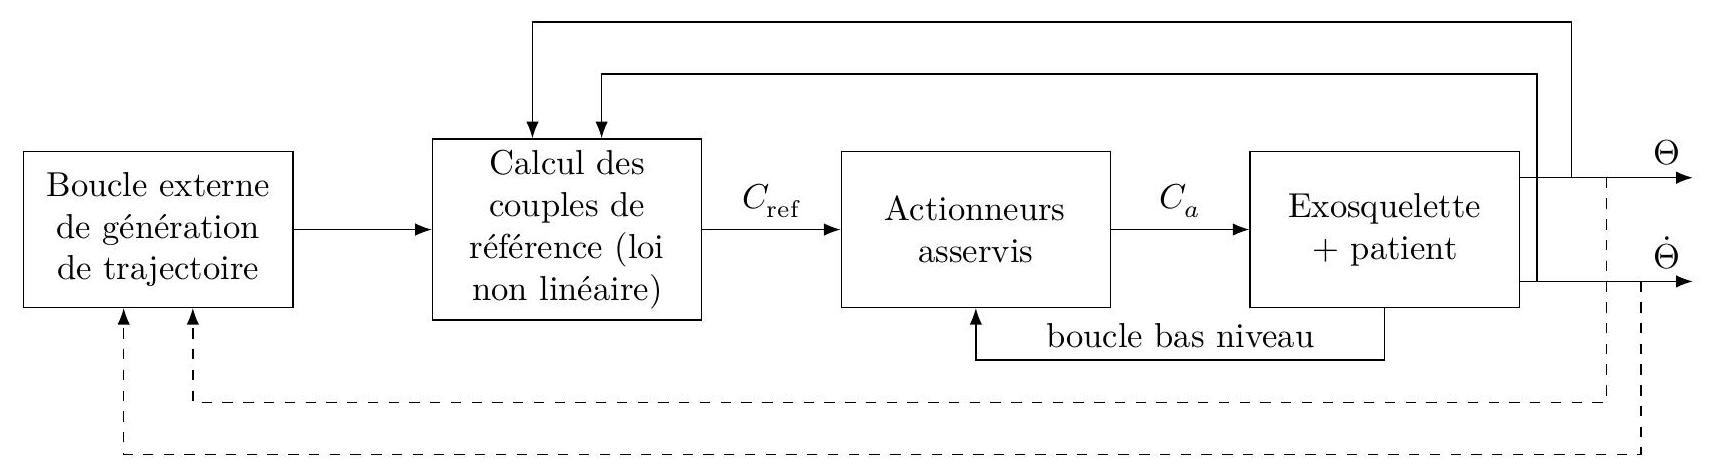
\includegraphics[max width=\textwidth]{2023_05_12_54c6a64d2ffce28d5c72g-07}
\end{center}

Figure 9 Détail de la structure de commande choisie

L'élaboration de la loi de commande de l'exosquelette se déroule alors en deux étapes:

\begin{itemize}
  \item l'asservissement en couple des actionneurs (boucle bas niveau) est réalisé en négligeant l'influence des éventuels couplages entre les axes. L'influence de cet asservissement sur la dynamique de l'exosquelette et la validité de cette approche sont étudiées. L'objectif de cette boucle bas niveau est de générer sur l'exosquelette des couples identiques aux couples de référence ;

  \item le calcul des couples de référence est réalisé par une boucle interne non linéaire.

\end{itemize}

\section{A - Conception de l'asservissement en couple d'un actionneur}
\section{- Objectif}
Élaborer l'asservissement du couple généré par un actionneur, puis le valider par une analyse de son effet sur l'exosquelette.

Lors des phases de rééducation, alors que le patient doit fournir un effort sous le contrôle du thérapeute, l'exosquelette doit réagir de façon totalement transparente pour le patient. En effet, l'exosquelette doit aider le patient, ou lutter contre les actions du patient, selon le protocole choisi par le thérapeute, et cela sans aucun à-coup. Ce constat implique que le temps de réponse de l'actionneur concerné par la phase rééducative doit être inférieur au temps de réponse physiologique du patient. La grande polyvalence de l'exosquelette a contraint les ingénieurs à choisir un temps de réponse de l'asservissement en couple de l'ordre de $0,1 \mathrm{~ms}$. L'objectif de cette partie est donc de concevoir l'asservissement du couple généré par les actionneurs et de vérifier si son action est bien transparente pour le patient.

\section{III.A.1) Modèle dynamique d'un axe}
Dans le but de concevoir l'asservissement du couple généré par un actionneur, il est nécessaire de déterminer le modèle dynamique de l'axe correspondant.

On considère le cas de l'ensemble \{pied+tibia\} 3, mis en mouvement par un actionneur placé sur la cuisse 2, supposée fixe et verticale $\left(\theta_{1}=0\right)$. L'influence des caractéristiques d'inertie et masse de l'actionneur est négligeable devant celle de l'ensemble \{pied+tibia\} 3. L'action mécanique exercée par le patient au niveau de l'articulation du genou est notée $C_{\text {genou }}$, celle exercée par l'actionneur sur l'axe de genou est notée $C_{2}$.

Q 14. Déterminer l'expression de l'accélération du point $G_{3}$ appartenant à l'ensemble \{pied+tibia\} 3 dans son mouvement par rapport à la cuisse 2 en fonction de $L_{0}, \theta_{2}$ et ses dérivées.

Q 15. Par application du théorème du moment dynamique à l'ensemble \{pied+tibia 3 au point B, projeté suivant la direction $\vec{x}_{1}$, donner l'expression de $C_{2}$ sous la forme :

$$
C_{2}=A_{\mathrm{eq}} \ddot{\theta}_{2}+C_{r}
$$

Préciser les expressions de $A_{\text {eq }}$ en fonction de $I_{x 3}, m_{3}, L_{0}$ et de $C_{r}$ en fonction de $C_{\text {genou }}, m_{3}, L_{0}, \alpha$ et $\theta_{2}$. Faire l'application numérique pour $A_{e q}$.

\section{III.A.2) Élaboration de la commande en couple de l'actionneur}
En exploitant le modèle dynamique précédent, le correcteur de la chaine d'asservissement en couple de l'actionneur doit être déterminé de façon à vérifier le cahier des charges ci-dessous :

\begin{center}
\begin{tabular}{|c|c|c|}
\hline
\multirow{2}{*}{Stabilité} & \multicolumn{2}{|c|}{Réponse à un échelon de consigne} \\
\cline { 2 - 3 }
 & Rapidité & Précision \\
\hline
régime apériodique critique & $t_{r, 5 \%}=0,1 \mathrm{~ms}( \pm 10 \%)$ & écart en régime permanent inférieur à $1 \%$ \\
\hline
\end{tabular}
\end{center}

L'actionneur utilisé est un ensemble motoréducteur. Le schéma-bloc présentant la structure de la commande utilisée et le procédé est présenté en annexe C avec :

\begin{itemize}
  \item $R_{m}=2,28 \Omega$

  \item $L_{m}=0,49 \mathrm{mH}$

\end{itemize}

$-k_{i}=k_{e}=0,89 \mathrm{~N} \cdot \mathrm{m} \cdot \mathrm{A}^{-1}$

\begin{itemize}
  \item $r$ rapport de transmission du motoréducteur $\left(r=\frac{1}{100}\right)$;

  \item $A_{\text {eq }}=2,0 \mathrm{~kg} \cdot \mathrm{m}^{2}$, quel que soit le résultat obtenu à la question 15 ;

  \item $C_{\text {pert }}$ couple de perturbation (correspondant à $C_{r}$ rapporté sur l'axe de l'actionneur);

  \item $C_{\text {ref }}$ couple de consigne désiré en sortie de l'actionneur ;

\end{itemize}

$-K_{\text {capi }}=1 \mathrm{~V} \cdot \mathrm{A}^{-1}$.

Pour la suite de cette partie, les conditions initiales sont considérées nulles et la synthèse du correcteur de type proportionnel-intégral se fait en considérant $C_{\text {pert }}=0$ :

$$
C_{i}(p)=K \frac{1+T p}{p}
$$

Q 16. Calculer, en donnant les expressions littérales de $K_{c}, T_{c}$, $\xi_{c}$ et $\omega_{c}$, l'expression de la fonction de transfert $H_{C}(p)=\frac{C_{m}(p)}{C_{r e f}(p)}$ sous la forme :

$$
H_{C}(p)=K_{c} \frac{1+T_{c} p}{1+2 \xi_{c} \frac{p}{\omega_{c}}+\left(\frac{p}{\omega_{c}}\right)^{2}}
$$

Pour simplifier la synthèse du correcteur, l'influence du zéro de $H_{C}(p)$ n'est pas prise en compte.

Q 17. Déterminer l'expression littérale, puis la valeur numérique, de $K$ afin de respecter le cahier des charges en termes de rapidité (rappel : $t_{r, 5 \%} \omega_{c} \approx 5$ pour un régime apériodique critique).

Q 18. Déterminer l'expression littérale, puis la valeur numérique, de $T$ afin de respecter le cahier des charges en termes de stabilité.

Q 19. Déterminer l'expression littérale, puis la valeur numérique, de $K_{1}$ afin d'obtenir $K_{C}=r$ pour $H_{C}(p)$. Justifier la volonté d'obtenir cette valeur de gain pour $H_{C}(p)$.

La figure 10 présente l'évolution temporelle de $C_{2}$, pour une entrée de type échelon de $1 \mathrm{~N} \cdot \mathrm{m}$.
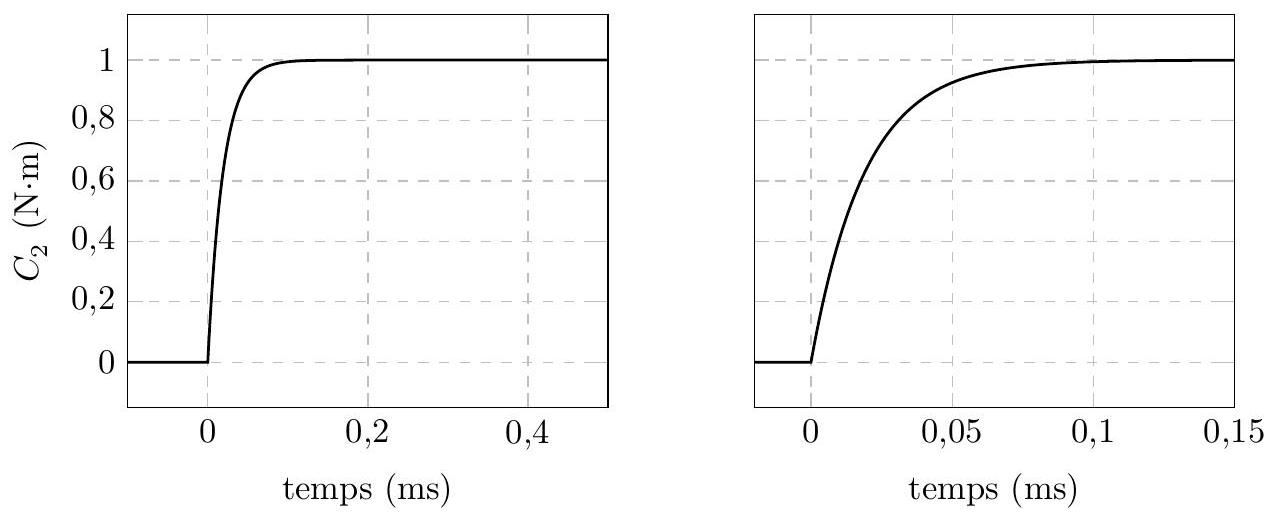
\includegraphics[max width=\textwidth, center]{2023_05_12_54c6a64d2ffce28d5c72g-08}

Figure 10 Réponse indicielle en couple de l'actionneur (agrandissement à droite)

Q 20. À partir de la figure 10, discuter du respect des exigences de l'asservissement en couple.

\section{III.A.3) Vérification de la cohérence de la commande en couple sur l'exosquelette}
La conception de l'asservissement du couple de l'actionneur a été réalisée sans prendre en compte les couplages entre les axes mis en évidence à la partie précédente. Afin de vérifier le comportement de cette commande une fois les axes couplés, il est nécessaire de considérer le réglage obtenu, mais en tenant compte de la dynamique globale de l'exosquelette déterminée dans la partie II comprenant le couplage entre les axes.

La figure 11 présente les réponses indicielles (entrée de type échelon de $1 \mathrm{~N} \cdot \mathrm{m}$ ) de la position angulaire $\theta_{2}$ pour le modèle dynamique de l'exosquelette pris seul (noté Mod1) et le modèle dynamique de l'exosquelette associé à ses actionneurs avec l'asservissement en couple élaboré précédemment (noté Mod2), ainsi que l'écart angulaire entre ces deux modèles.

La figure 12 présente les réponses indicielles (entrée de type échelon de $1 \mathrm{~N} \cdot \mathrm{m}$ ) du couple $C_{2}$ pour le modèle dynamique de l'exosquelette associé à ses actionneurs avec l'asservissement en couple élaboré précédemment (Mod2) et pour le modèle dynamique de l'axe pris seul (noté Mod3), ainsi que l'écart en couple entre ces deux modèles.
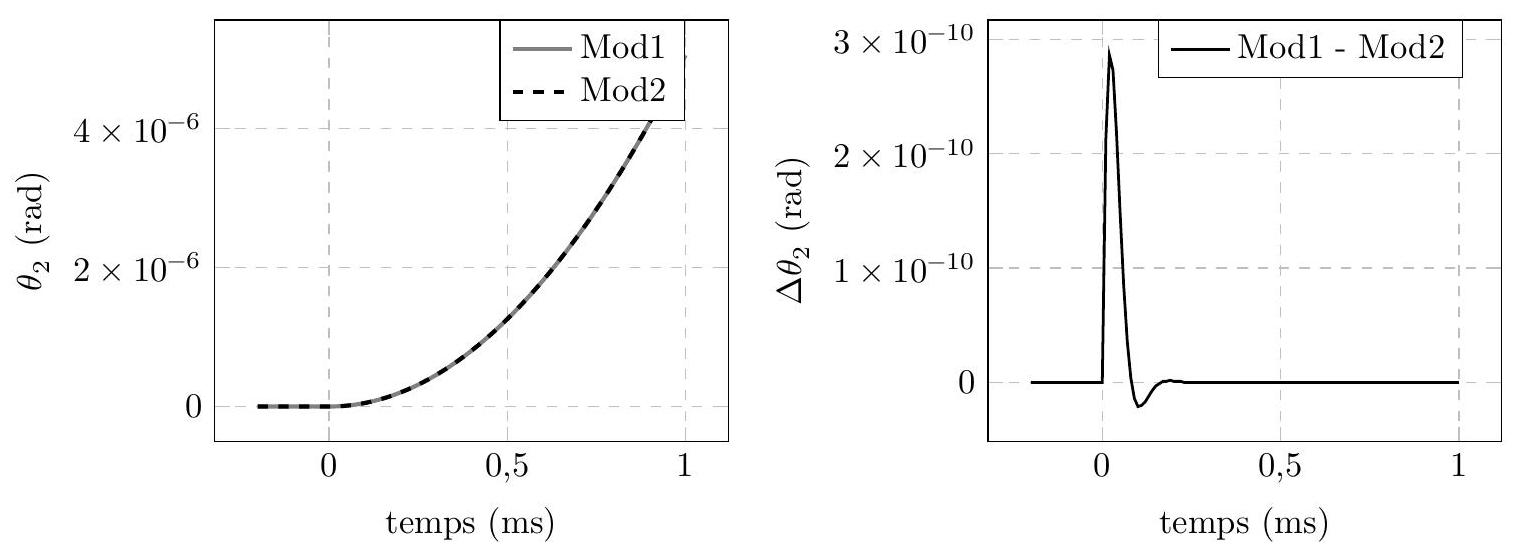
\includegraphics[max width=\textwidth, center]{2023_05_12_54c6a64d2ffce28d5c72g-09}

Figure 11 Réponse indicielle angulaire des modèles Mod1 et Mod2 et écart de position angulaire
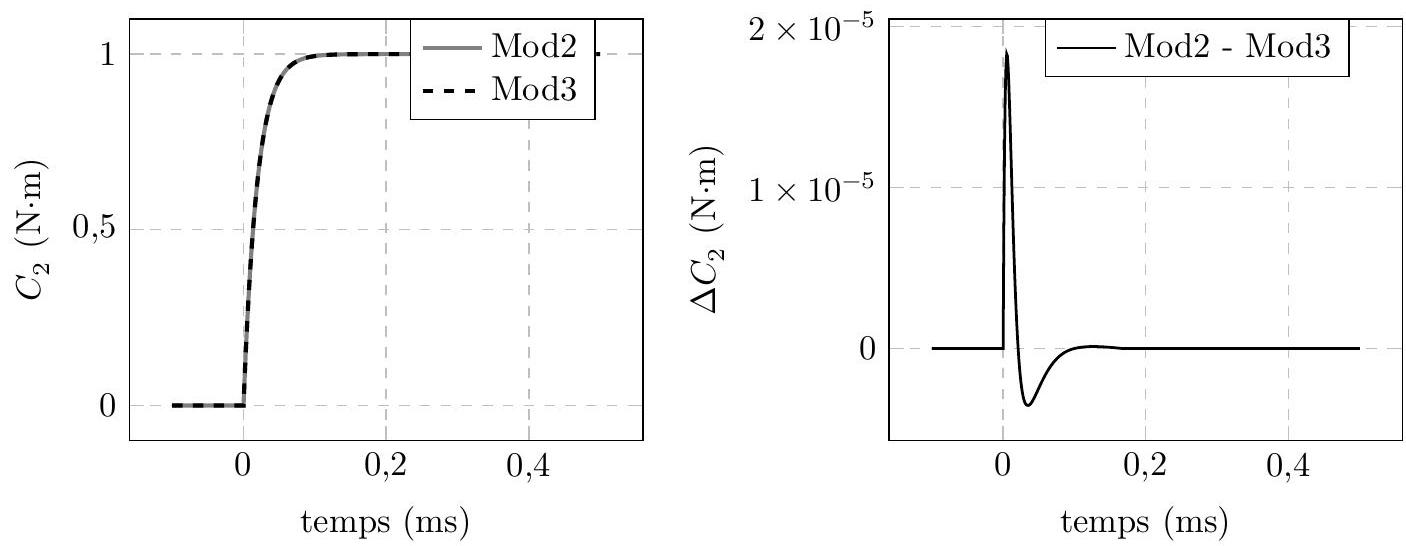
\includegraphics[max width=\textwidth, center]{2023_05_12_54c6a64d2ffce28d5c72g-09(1)}

Figure 12 Réponse indicielle en couple des modèles $\operatorname{Mod} 2$ et Mod3 et écart de couple

Q 21. À partir des figures 11 et 12, conclure sur la possibilité de considérer l'asservissement en couple comme amenant une action transparente pour le patient.

Cet asservissement en couple permet, sur la figure 9, de considérer que si les couples de commande $C_{\text {ref }}$ sont générés correctement, alors les couples $C_{a}$ appliqués sur les articulations permettront au patient d'avoir la trajectoire voulue. L'élaboration de la loi de commande non linéaire peut se faire en considérant directement des commandes en couples pour chacun des axes, c'est-à-dire en considérant la réponse en couple des actionneurs comme unitaire.

\section{III.B - Synthèse de la loi de commande de l'exosquelette}
\section{Objectif}
Élaborer une loi de commande en phase de rééducation à la proprioception de la verticalité et de la marche, et en phase de renforcement musculaire.

Les actionneurs ayant été asservis en couple, la loi de commande est réalisée pour générer des consignes en couple. Ces consignes doivent permettre à l'exosquelette de réaliser les deux types d'exercices désirés :

\begin{itemize}
  \item le renforcement musculaire. Cette partie étudie la synthèse d'une loi de commande pour cet exercice ;

  \item la rééducation à la proprioception de la verticalité et de la marche. Cette partie analyse une loi de commande donnée pour cet exercice. III.B.1) Formulation d'un modèle pour la synthèse de la loi de commande

\end{itemize}

Le modèle dynamique de l'exosquelette, déterminé à l'aide de la partie II.A question 11, est de la forme :

$$
M_{1}(\Theta, \dot{\Theta}) \ddot{\Theta}+M_{2}(\Theta, \dot{\Theta}) \dot{\Theta}+C(\Theta, \dot{\Theta})+M_{3}(\Theta, \dot{\Theta}) C_{p}=C_{\mathrm{ref}}
$$

Dans cette équation, on note :

$-\Theta=\left(\begin{array}{c}\theta_{1} \\ \theta_{2}\end{array}\right)$ les coordonnées angulaires des articulations ;

\begin{itemize}
  \item $C$, la matrice colonne correspondant aux effets de la pesanteur ;
\end{itemize}

$-C_{p}=\left(\begin{array}{c}C_{\text {hanche }} \\ C_{\text {genou }}\end{array}\right)$ les actions mécaniques exercées par le patient ;

$-C_{\mathrm{ref}}=\left(\begin{array}{l}C_{1} \\ C_{2}\end{array}\right)$, les actions mécaniques de consigne (générées par les actionneurs dont les boucles d'asservissement en couple sont considérées comme infiniment rapides).

\begin{center}
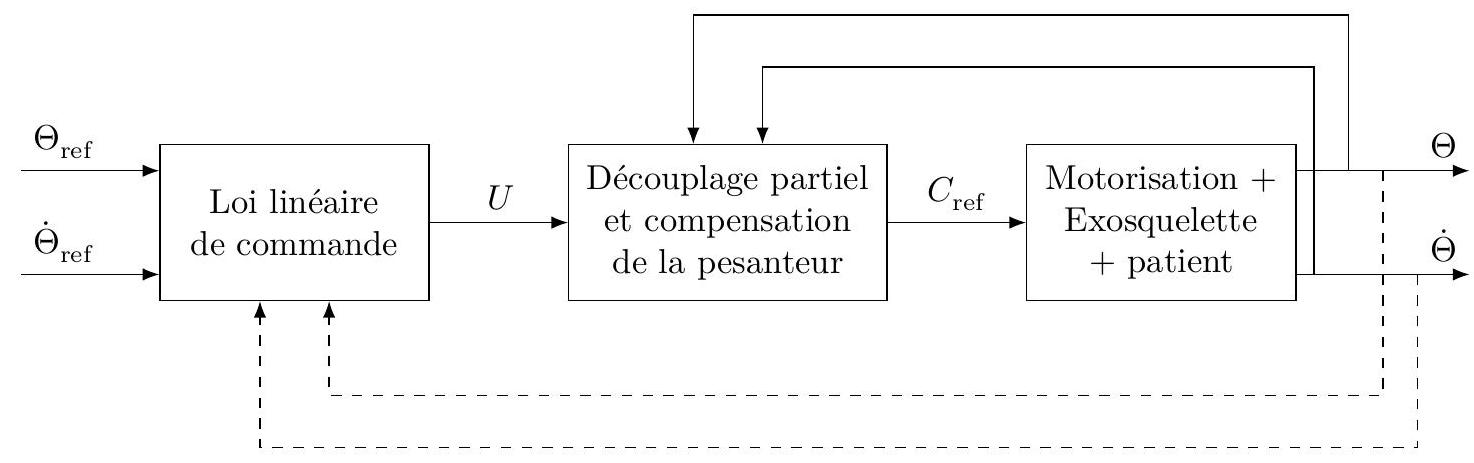
\includegraphics[max width=\textwidth]{2023_05_12_54c6a64d2ffce28d5c72g-10}
\end{center}

Figure 13 Structure de la loi de commande couplée

La structure de la loi de commande choisie, présentée figure 13, est réalisée selon deux boucles :

\begin{itemize}
  \item une boucle externe linéaire ;

  \item une boucle interne non linéaire, devant permettre le découplage partiel du modèle dynamique et la compensation de la pesanteur, qui détermine le couple $C_{\text {ref }}$ par la relation :

\end{itemize}

$$
C_{\mathrm{ref}}=M_{1}(\Theta, \dot{\Theta}) U+M_{2}(\Theta, \dot{\Theta}) \dot{\Theta}+C(\Theta, \dot{\Theta})
$$

où $U=\left(\begin{array}{l}U_{1} \\ U_{2}\end{array}\right)$ sont les commandes issues du correcteur linéaire de la boucle externe.

On note, de plus, les consignes de positions angulaires sous la forme $\Theta_{\text {ref }}=\left(\begin{array}{c}\theta_{1, \text { ref }} \\ \theta_{2, \text { ref }}\end{array}\right)$.

En utilisant la loi correspondant à la boucle interne, le modèle dynamique peut s'écrire sous la forme :

$$
\ddot{\Theta}=U+N\left(\Theta, \dot{\Theta}, C_{p}\right)
$$

où $N\left(\Theta, \dot{\Theta}, C_{p}\right)=M(\Theta, \dot{\Theta}) C_{p}$.

Q 22. Préciser l'expression de la matrice $M$ introduite précédemment en fonction de $M_{1}$ et $M_{3}$.

Afin de réaliser cette loi de commande, il est nécessaire de linéariser le modèle dynamique autour du point de fonctionnement. Ce point de fonctionnement est défini par :

$-\Theta_{0}=\left(\begin{array}{c}\theta_{1,0} \\ \theta_{2,0}\end{array}\right)$, les coordonnées angulaires des articulations au point de fonctionnement ;

\begin{itemize}
  \item $C_{p, 0}=\left(\begin{array}{c}C_{\text {hanche }, 0} \\ C_{\text {genou }, 0}\end{array}\right)$, les actions mécaniques exercées par le patient au point de fonctionnement;
\end{itemize}

$-u=\left(\begin{array}{l}u_{1} \\ u_{2}\end{array}\right)$, les variations des grandeurs de commandes autour de $U_{0}=\left(\begin{array}{c}U_{1,0} \\ U_{2,0}\end{array}\right)$;

$-\tilde{\theta}=\left(\begin{array}{c}\tilde{\theta}_{1} \\ \tilde{\theta}_{2}\end{array}\right)$, les variations des positions angulaires autour de $\Theta_{0}=\left(\begin{array}{c}\theta_{1,0} \\ \theta_{2,0}\end{array}\right)$;

$-c_{p}=\left(\begin{array}{c}c_{\text {hanche }} \\ c_{\text {genou }}\end{array}\right)$, les variations des actions mécaniques exercées par le patient autour de $C_{p, 0}=\left(\begin{array}{c}C_{\text {hanche }, 0} \\ C_{\text {genou }, 0}\end{array}\right)$.


\end{document}